\section{Abhängigkeiten}
\begin{frame}
	\frametitle{Beispiel Programm}
	Ein einfaches Programm aus 3 Modulen
    \begin{itemize}
      \item<2->[] 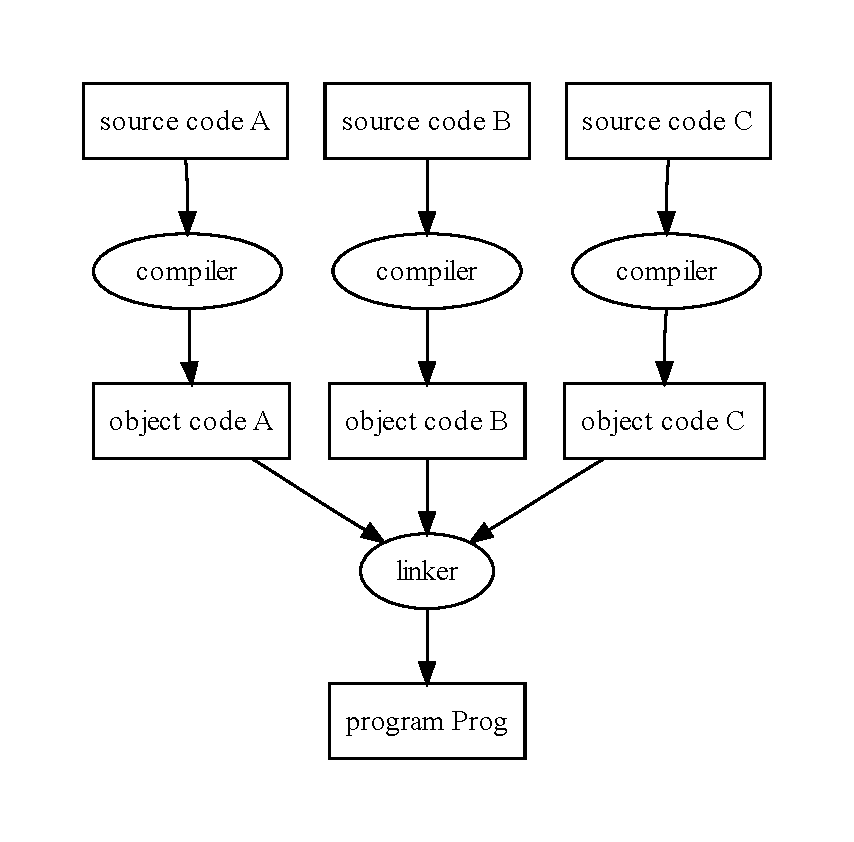
\includegraphics[scale=0.5]{prog1.pdf}      
    \end{itemize}

\end{frame}

\begin{frame}
	\frametitle{Beispiel Programm2}
	Ein anderes einfaches Programm aus 3 Modulen, mit mehr Abhängigkeiten
    \begin{itemize}
      \item<2->[] 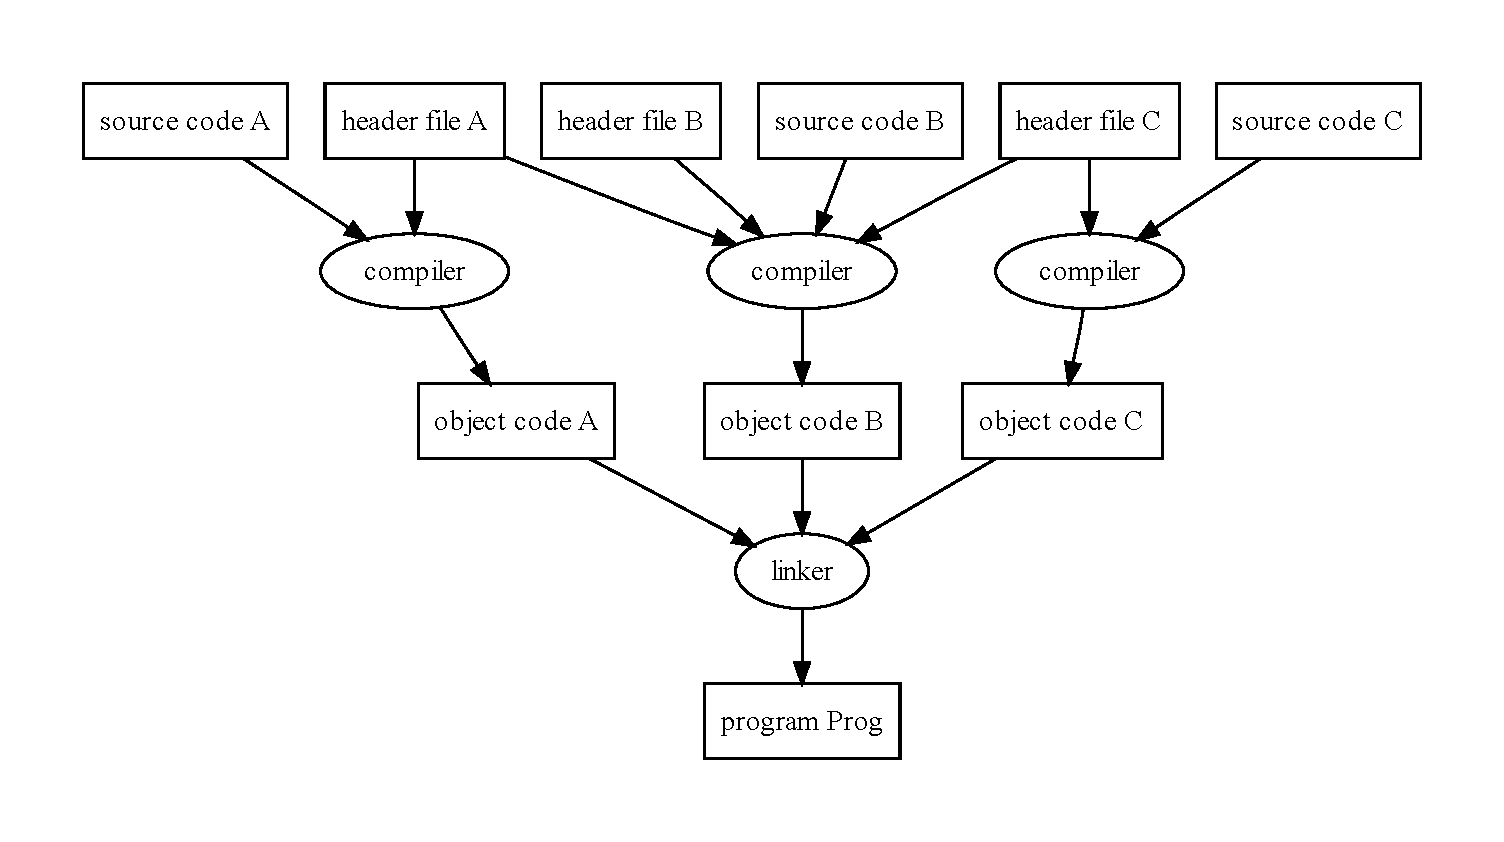
\includegraphics[scale=0.41]{prog2.pdf}      
    \end{itemize}
\end{frame}

\begin{frame}
	\frametitle{Abhängigkeiten Programm2}
	Abhängigkeiten in Programm2
    \begin{itemize}
      \item<2->[] 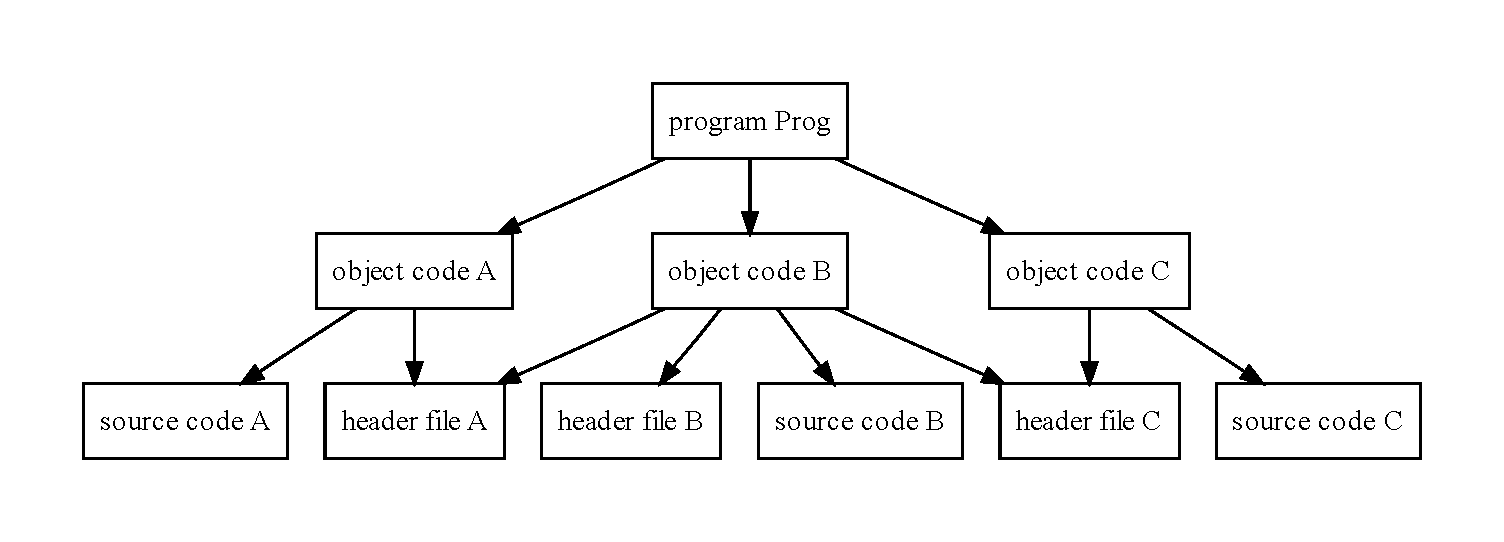
\includegraphics[scale=0.41]{prog2-dep.pdf}      
    \end{itemize}
\end{frame}


\begin{frame}
	\frametitle{Abhängigkeiten Programm2}
	Folgen einer Änderung in \textit{header file A}
    \begin{itemize}
      \item<2->[] 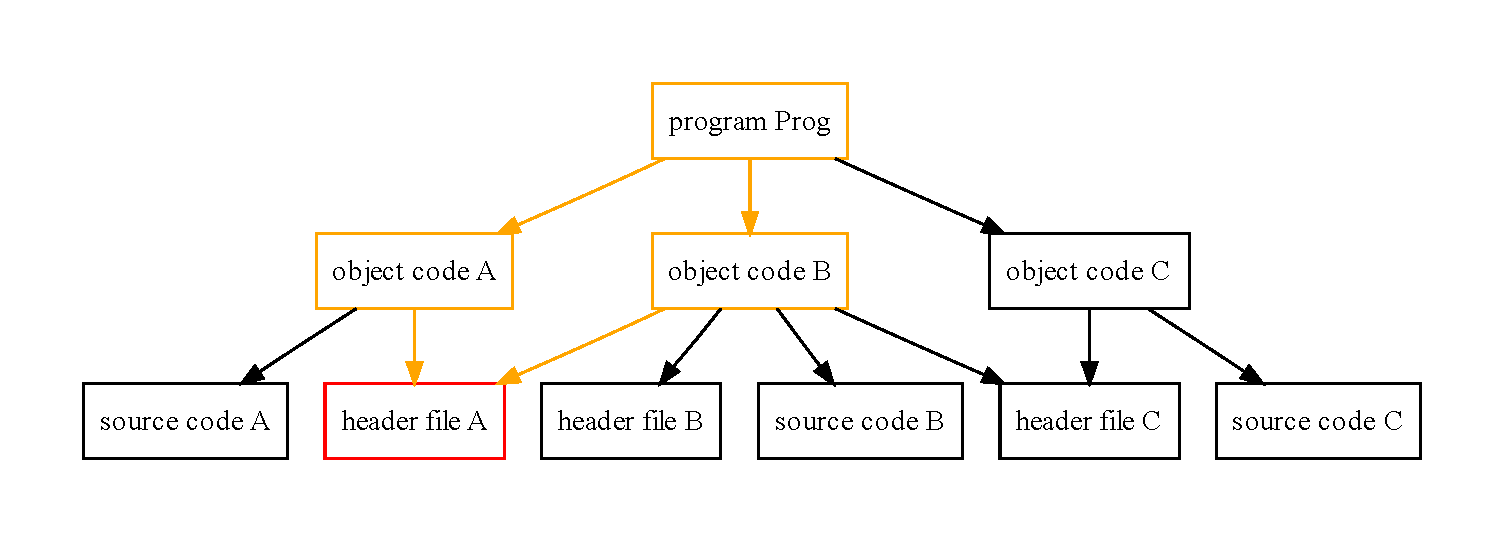
\includegraphics[scale=0.41]{prog2-dep-hl.pdf}      
    \end{itemize}
\end{frame}

\begin{frame}
	\frametitle{Was Make für dich tut}
    \begin{itemize}
      \item<2-> \large{Prüfung des Dateialters (mit Hilfe des Timestamps des Dateisystems)}
      \item<3-> \large{(neu) Erzeugen der Dateien, deren Abhängigkeiten sich geändert haben}       
    \end{itemize}
\end{frame}

\begin{frame}
	\frametitle{Was du tun must}
    \begin{itemize}
      \item<2-> \large{Make die Abhängigkeitsverhältnisse mitteilen (welche Datei hängt von wecher ab)}
      \item<3-> \large{Make mitteilen wie die Dateien zu bauen sind} 
    \end{itemize}
\end{frame}